\chapter{从等效原理到张量}

广义相对论通常简称为GR，尽管狭义相对论很少被称为SR。这个缩写不如从头开始的决定重要。最直接的路线是爱因斯坦走过的路线：从一个简单到在电梯里就能感受到的物理观察出发，不断推进它，直到其后果变得不可避免，然后才引入几何。

第一个观察是等效原理。引力和加速度在局部是不可区分的。局部这个词最终将承担这一陈述几乎全部的负担。然而，在限定它之前，我们应该先看看未加限定的陈述已经能做什么。

\section{电梯作为坐标变换}

教科书常常用火箭飞船代替爱因斯坦的电梯。这里电梯更可取，因为它的加速度是熟悉的。设\(z\)在附着于地面的参考系中测量高度，设\(z'\)从电梯地板测量高度。如果地板的高度为\(L(t)\)，同一事件具有坐标
\begin{equation}
 z'=z-L(t),\qquad t'=t,\qquad x'=x.
\label{eq:elevator-map}
\end{equation}
水平坐标不变，因为电梯不侧向滑动。取\(t'=t\)是故意暂时压制狭义相对论。

\begin{classroomqa}
\audiencequestion{一门广义相对论课程怎么能以忽略狭义相对论开始呢？}
\lecturerresponse{存在这样一个区域，其中引力起作用而所有速度与\(c\)相比仍然很小。因此，引力--加速度的联系可以在牛顿力学中孤立出来，然后再与闵可夫斯基几何结合。这是一个分阶段的安排，而不是声称最终理论是非相对论性的。\lecturetimestamp{00:05:33}}
\end{classroomqa}

对于两个惯性参考系，电梯匀速运动，
\begin{equation}
 L(t)=vt,\qquad z'=z-vt.
\label{eq:galilean-elevator}
\end{equation}
原点被选为在\(t=0\)时重合。板书将电梯草图保留在所有三个坐标关系旁边，以便符号永远不会失去其物理意义。

\begin{figure}[H]
\centering
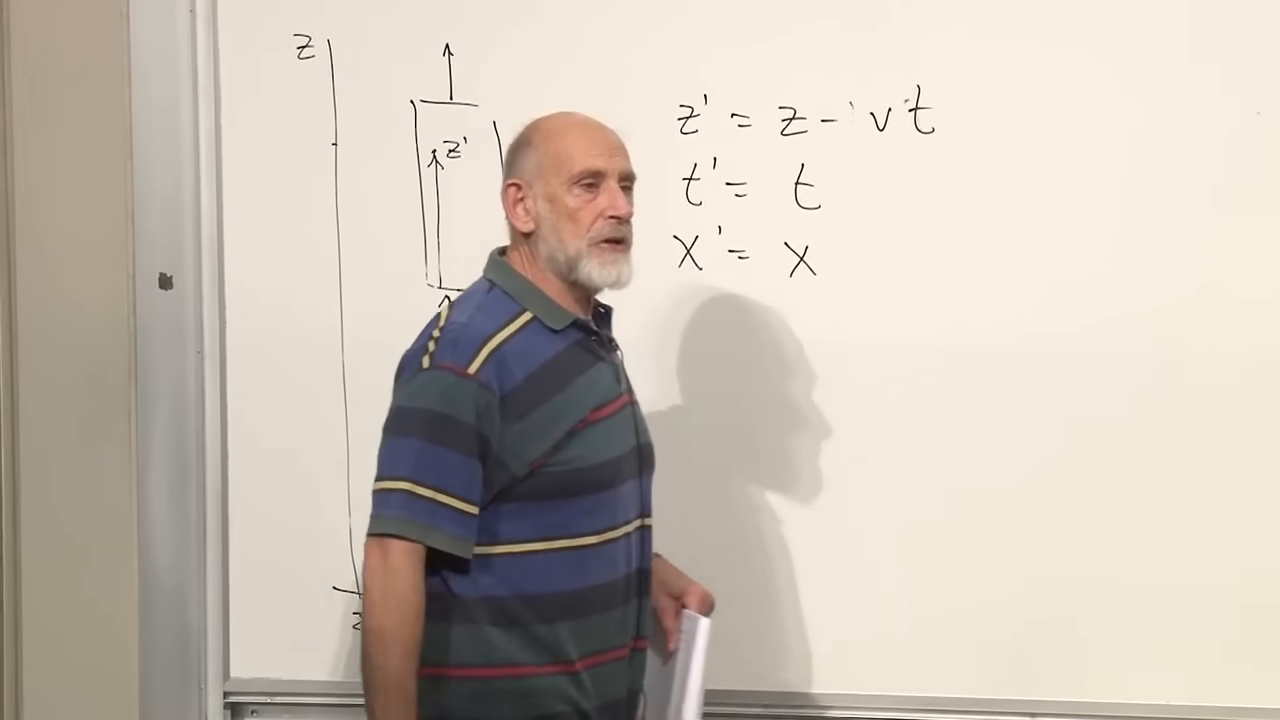
\includegraphics[width=\linewidth]{lecture_01_figure_01.png}
\caption{匀速特化\(L(t)=vt\)之后的电梯坐标。}
\par\smallskip
\textit{讲义帧：00：09：10。}
\end{figure}

只考虑牛顿定律的竖直分量，
\begin{equation}
 F=m\ddot z.
\label{eq:newton-unprimed}
\end{equation}
力可以来自绳子、电场或任何其他普通相互作用。对\eqref{eq:galilean-elevator}求两次导数得到
\(\ddot z'=\ddot z\)，因此
\begin{equation}
 F=m\ddot z'.
\label{eq:newton-primed-inertial}
\end{equation}
定律的形式不变。这个初等计算揭示了惯性参考系等效的实际内容：线性坐标变换将匀速运动变为匀速运动。

\begin{figure}[H]
\centering
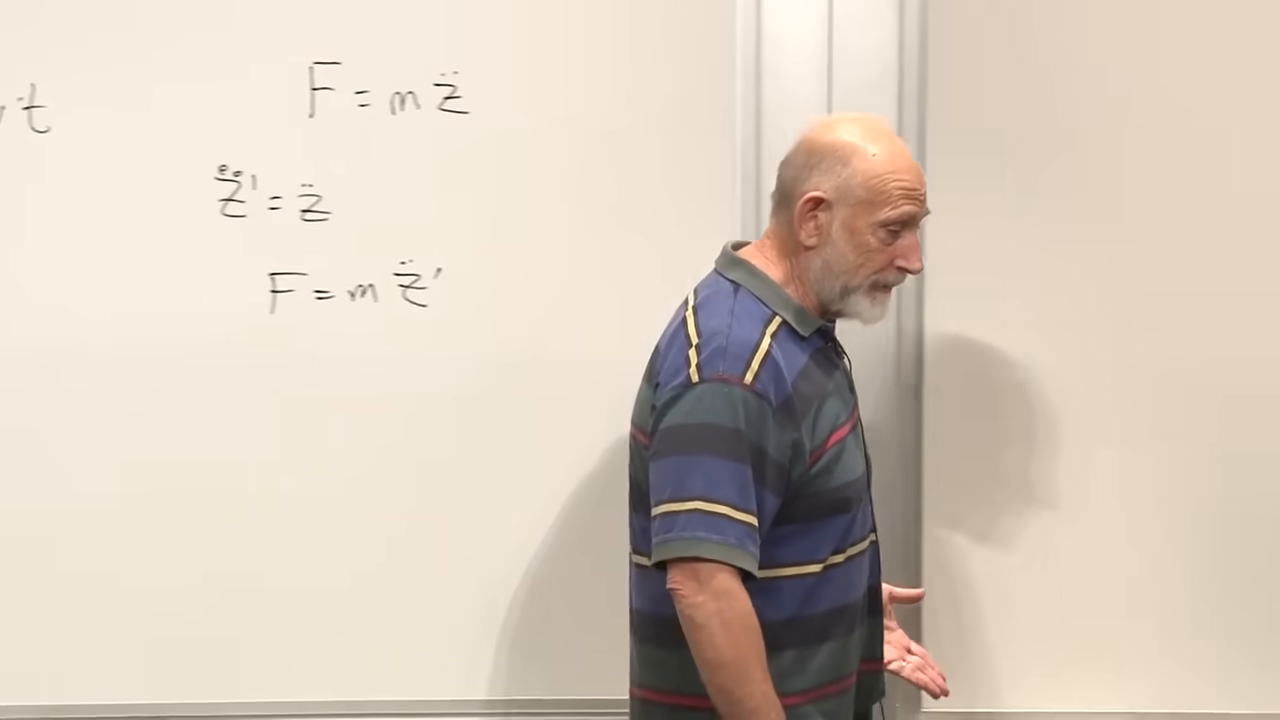
\includegraphics[width=\linewidth]{lecture_01_figure_02.png}
\caption{两个匀速运动坐标参考系中的牛顿方程。}
\par\smallskip
\textit{讲义帧：00：11：50。}
\end{figure}

现在让电梯以恒定\(g\)向上加速：
\begin{equation}
 L(t)=\frac12gt^2,\qquad
 \dot L=gt,\qquad
 \ddot L=g.
\end{equation}
坐标变换变为
\begin{equation}
 z'=z-\frac12gt^2,
\qquad
 \ddot z'=\ddot z-g.
\label{eq:accelerated-map}
\end{equation}
代入牛顿定律得到
\begin{equation}
 F=m(\ddot z'+g),
\qquad
 m\ddot z'=F-mg.
\label{eq:fictitious-gravity}
\end{equation}
推导中包含一个有用的实时符号检查：\(+mg\)首先出现在加速度一侧，只有当移到力一侧时才变为\(-mg\)。最终方向在地板向上加速的参考系中是向下的。

\begin{figure}[H]
\centering
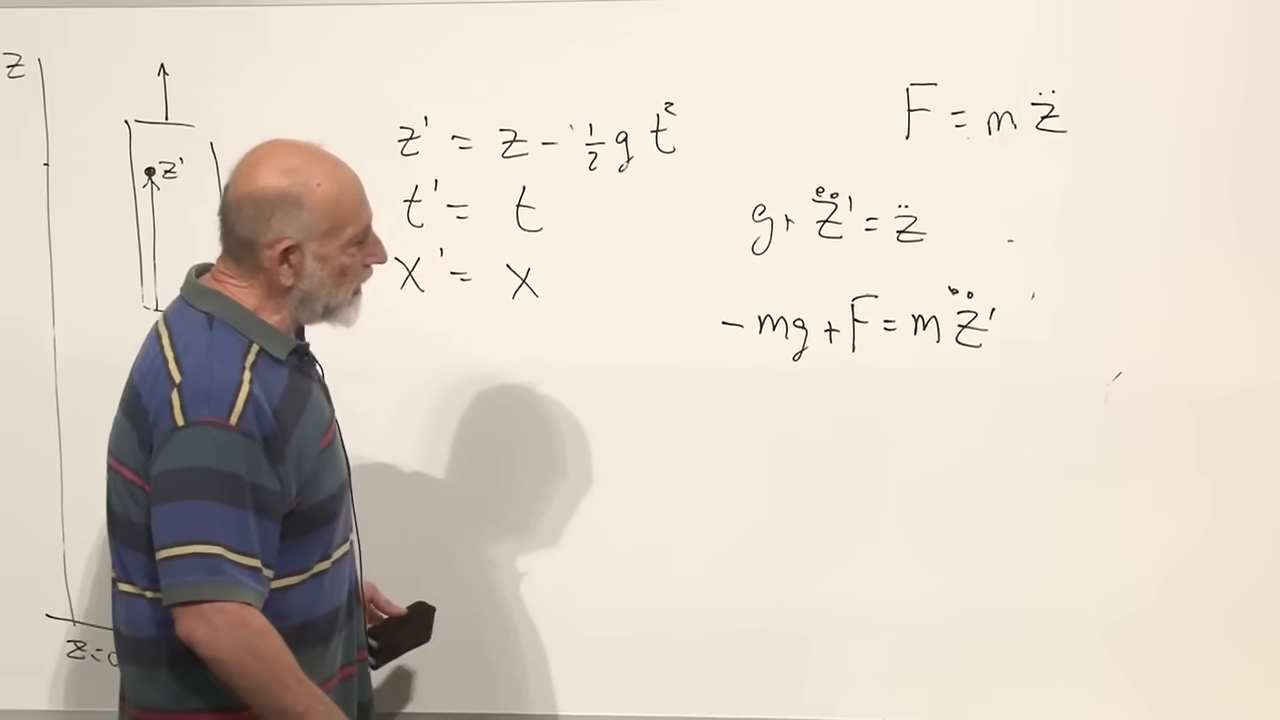
\includegraphics[width=\linewidth]{lecture_01_figure_03.png}
\caption{加速变换及由此产生的虚拟力\(-mg\)。}
\par\smallskip
\textit{讲义帧：00：15：35。}
\end{figure}

新项看起来像引力，原因很精确：它与质量成正比。由于惯性响应也与质量成正比，质量从运动方程中消去。自由落体无论其质量如何都遵循相同的轨迹。例如，在试验体近似中，地球的轨道由其位置和速度在太阳场中决定，而不是由地球自身的质量决定。

在爱因斯坦之前，这种相似性可以被当作奇闻而忽略。爱因斯坦反而将其提升为一条原理：没有任何局部力学实验能够区分均匀引力场和适当加速的参考系。

\section{直线、曲线坐标与光}

将\(t\)竖直绘制，\(z\)水平绘制。对于
\(z'=z-vt\)，恒定\(z'\)的线是平行直线。
直线世界线保持直线，因为坐标变换是线性的。

\begin{figure}[H]
\centering
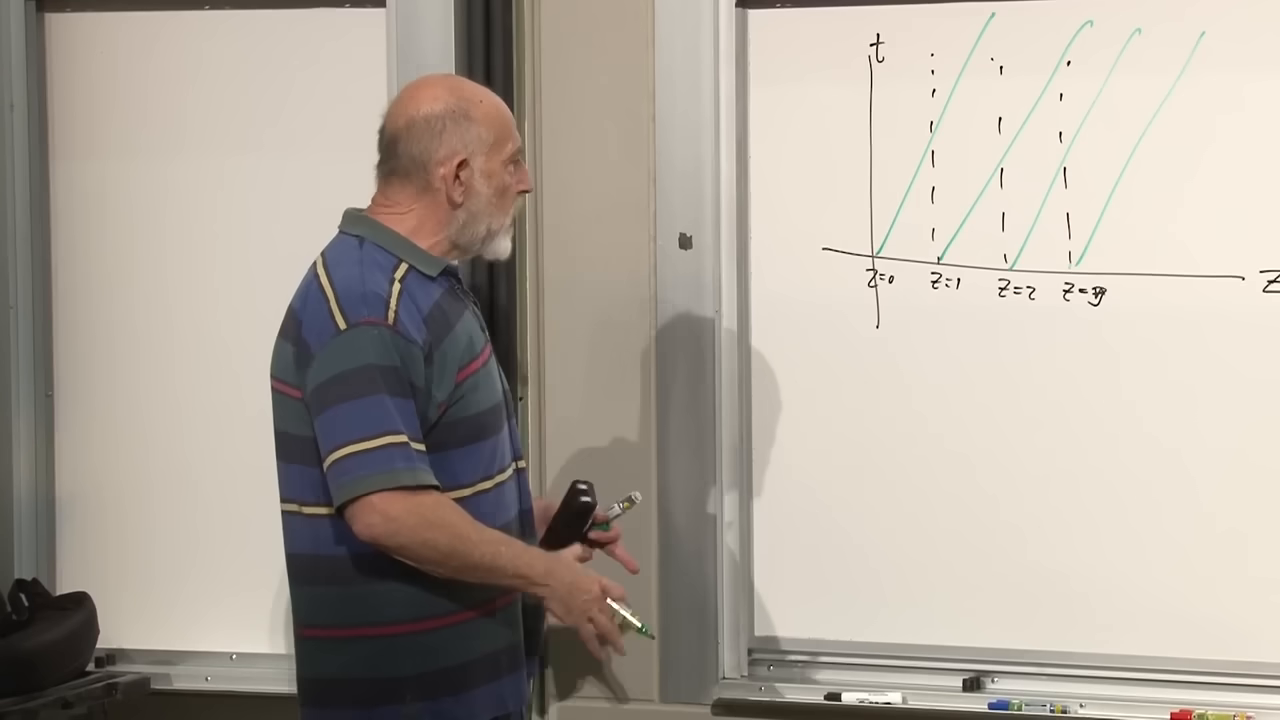
\includegraphics[width=\linewidth]{lecture_01_figure_04.png}
\caption{匀速运动坐标的线性时空网格。}
\par\smallskip
\textit{讲义帧：00：19：45。}
\end{figure}

对于加速映射，一条常\(z'\)线满足
\begin{equation}
 z=z'+\frac12gt^2.
\end{equation}
它是一条横躺的抛物线。将运动沿时间反向延伸，得到一部电梯：它一边下降一边减速，随后转向，然后向上加速。每一条相邻的常\(z'\)线都是同一条抛物线水平平移后的结果。

\begin{figure}[H]
\centering
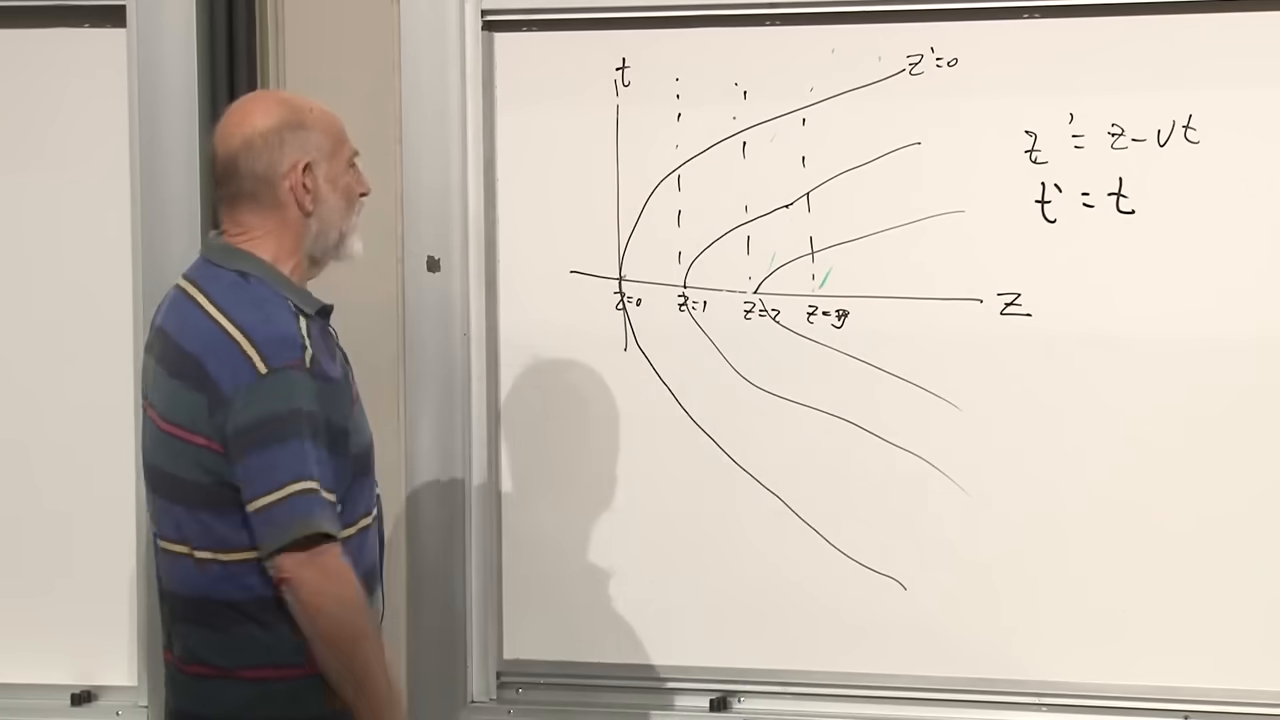
\includegraphics[width=\linewidth]{lecture_01_figure_05.png}
\caption{匀加速坐标系的常\(z'\)曲线。}
\par\smallskip
\textit{讲义帧：00：22：25。}
\end{figure}

这是第一条几何线索。狭义相对论使用线性洛伦兹变换，而线性洛伦兹变换把直线时空线变为直线时空线。要表示加速度，从而模仿引力，就需要时空坐标的曲线变换。

爱因斯坦用这个看似不起眼的论点回答了一个一点也不不起眼的问题：引力是否影响光？在\(t=0\)时，设电梯系与地面系彼此瞬时静止，并让一条水平光线穿过电梯。在未加速的参考系中，
\begin{equation}
 x=ct,\qquad z=0.
\end{equation}
利用\(z=z'+\tfrac12gt^2\)，同一条光线在电梯坐标中满足
\begin{equation}
 z'=-\frac12gt^2
    =-\frac{g}{2c^2}x^2.
\label{eq:accelerated-light}
\end{equation}
这条光线在惯性系中是直的，在加速系中是弯的。如果加速度与引力局域等价，那么引力场必定使光弯曲。这个论证在尚未写出引力场方程之前就确立了这个效应。

\begin{figure}[H]
\centering
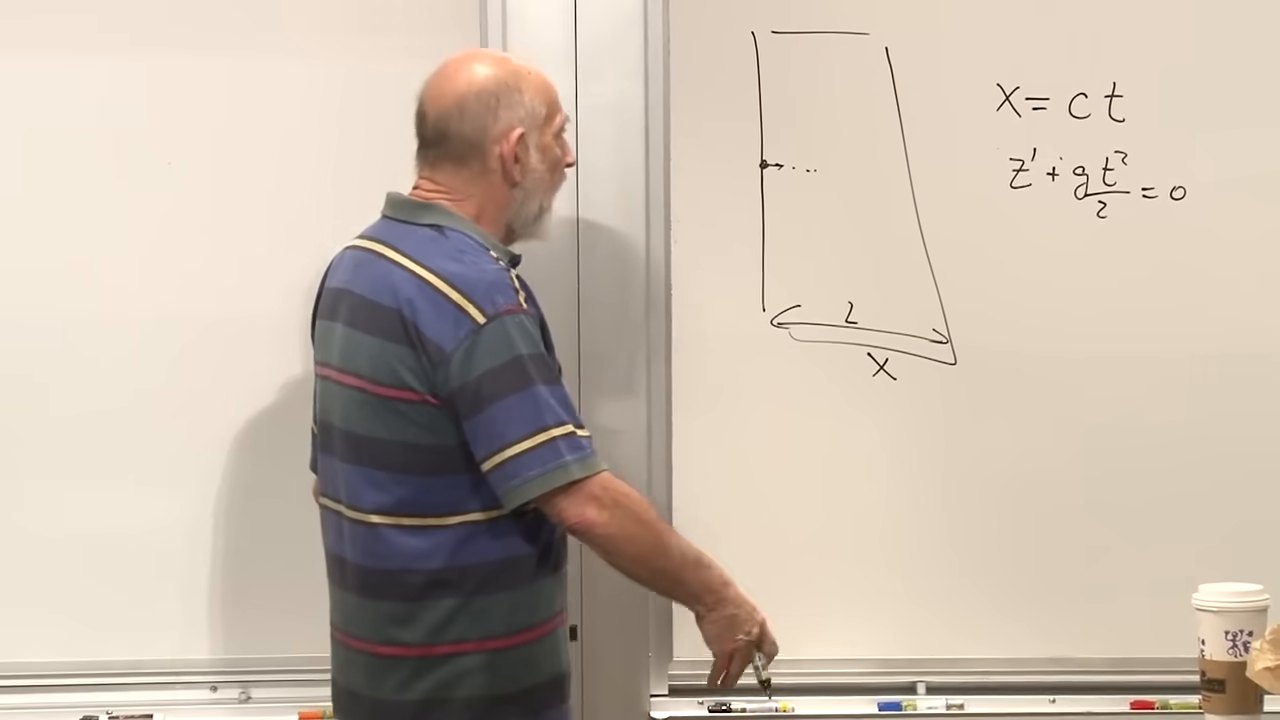
\includegraphics[width=\linewidth]{lecture_01_figure_06.png}
\caption{水平光线及其在加速系中的弯曲轨迹。}
\par\smallskip
\textit{讲义帧：00：28：10。}
\end{figure}

\section{无法被变换掉的东西}

加速系可以制造出一个表观的均匀引力场。但并不能由此推出每个引力场都是坐标的产物。恒星的场沿径向指向内部。一个靠近某一点的自由下落小实验室可以消除局域加速度，但同一个变换无法消除恒星四周各处的场。

\begin{figure}[H]
\centering
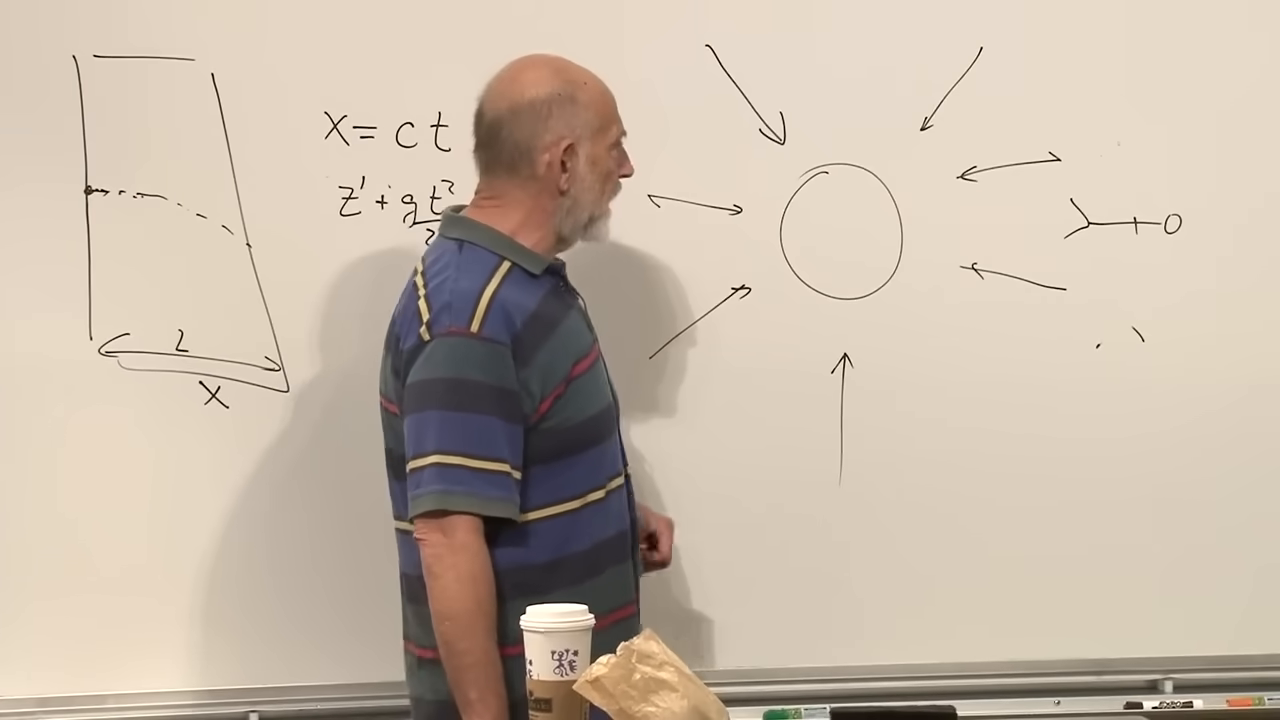
\includegraphics[width=\linewidth]{lecture_01_figure_07.png}
\caption{一个径向场和一个用来暴露潮汐加速度的延展下落物体。}
\par\smallskip
\textit{讲义帧：00：32：50。}
\end{figure}

障碍在于潮汐力。想象一个身高两千英里的人脚朝下下落。他的脚离源更近，加速得比头更强烈，因此他被拉伸。把他转成侧向，则两侧的向内方向具有彼此指向对方的分量，因此他被挤压。用牛顿力学的语言说，相隔\(\xi^j\)的相邻点获得相对加速度
\begin{equation}
 \delta a^i \simeq \partial_j g^i\,\xi^j.
\label{eq:newtonian-tide}
\end{equation}
坐标加速度可以被消除。一个延展的自由下落物体上的相对加速度则不能被消除。

\begin{classroomqa}
\audiencequestion{如果在头部和脚部分别用不同的火箭发动机，能否模拟这种拉伸，从而模拟潮汐场？}
\lecturerresponse{施加发动机当然可以使物体受力，但那是真实的非引力作用力，并且对物体各部分的作用不同。仅靠坐标变换无法在相邻的自由下落粒子之间产生不变的相对加速度。这一判据针对的是不受力的自由下落，而不是由各自火箭驱动的物体。
\lecturetimestamp{00:36:51}}
\end{classroomqa}

不过，弯曲坐标可以使虚构场显得相当复杂。一个参考系可以竖直加速，同时水平振荡，从而产生一个含两个分量的、依赖时间的表观场。就连普通的极坐标也提供了一个有启发性的例子。一个在笛卡儿直线坐标中沿直线运动的自由粒子，其\(r(t)\)先减小，达到最小半径，然后\(r(t)\)增大。只拿到\(r(t)\)和\(\theta(t)\)的人可能会推断存在一个向外的排斥力。在这些坐标的旋转变体中，会出现离心项和科里奥利项。它们与质量成正比，因此看起来像引力，但它们不会在自由下落物体上留下不变的潮汐应变。

\begin{classroomqa}
\audiencequestion{如果用角坐标或极坐标描述运动，会发生什么？}
\lecturerresponse{非线性的坐标描述使一条笔直的自由轨迹看起来像是被\(r=0\)排斥。那个有效离心力是一种坐标力。回到惯性笛卡儿系就把它去掉，并揭示出并不存在潮汐畸变。
\lecturetimestamp{00:37:56}}
\end{classroomqa}

\begin{figure}[H]
\centering
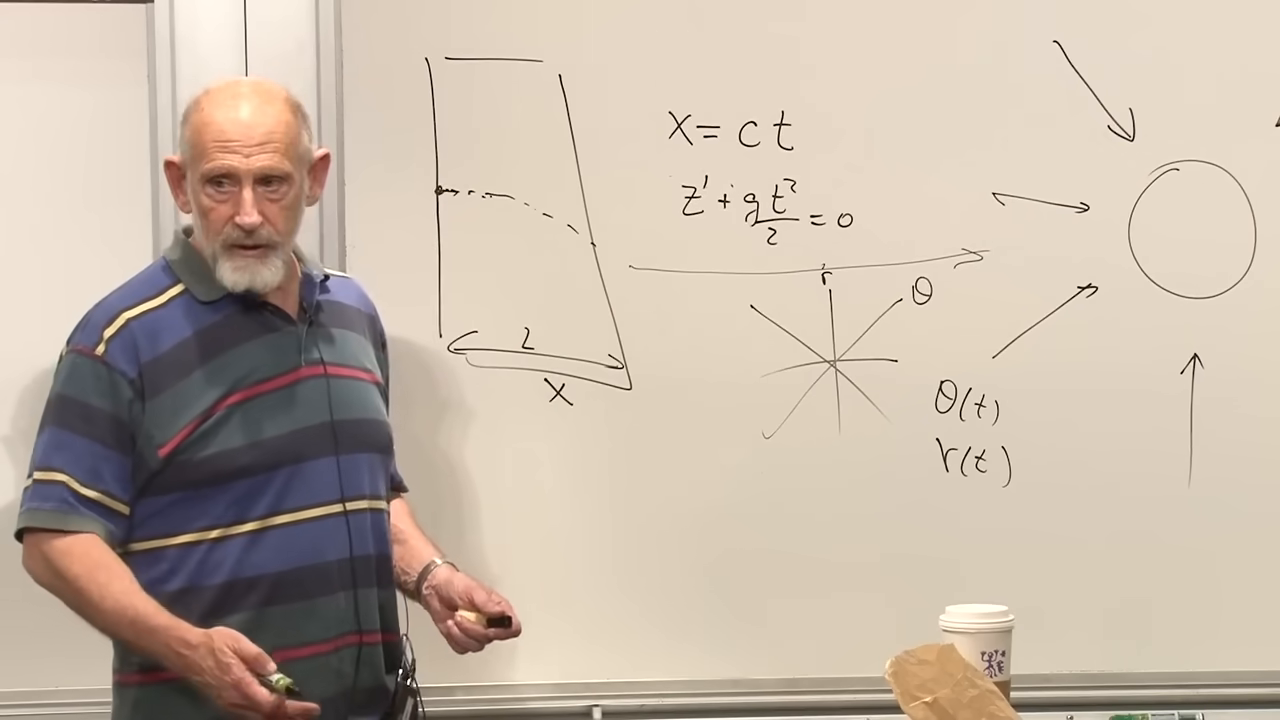
\includegraphics[width=\linewidth]{lecture_01_figure_08.png}
\caption{直线轨迹的极坐标描述，黑板上标出了\(r(t)\)和\(\theta(t)\)。}
\par\smallskip
\textit{讲义帧：00：40：20。}
\end{figure}

\begin{classroomqa}
\audiencequestion{多个引力体能否相互抵消，从而不留下任何潮汐力？}
\lecturerresponse{力可以在选定的点上抵消，但场值的抵消一般并不能抵消其空间导数。在任何一个源附近，邻近的轨迹仍然会获得不同的加速度。要真正不存在曲率，潮汐诊断量必须在整个区域内消失，而不仅仅是在某一点上净力为零。\lecturetimestamp{00:42:16}}
\end{classroomqa}

\begin{classroomqa}
\audiencequestion{如何在操作上测量潮汐力？}
\lecturerresponse{让一个延展物体，例如一块晶体，自由下落，并寻找使其在一个方向上被拉伸、在另一个方向上被压缩的应力和应变。这些形变是可测量的，并且不会因为坐标重新命名而消失。\lecturetimestamp{00:44:38}}
\end{classroomqa}

\begin{classroomqa}
\audiencequestion{一个两千英里高的人坐在旋转木马上，会感受到径向的潮汐效应吗？}
\lecturerresponse{被绑在旋转木马上的人会感受到支撑力，确实可能会头痛。但测试物体必须是自由下落的。它的轨迹在旋转坐标中看起来很复杂，但在惯性系中仍然是一条无应力的直线轨迹，因此不变的潮汐力为零。
\lecturetimestamp{00:45:07}}
\end{classroomqa}

\begin{classroomqa}
\audiencequestion{能否将下落物体倾斜，使拉伸和挤压相互抵消？}
\lecturerresponse{没有任何单一取向能消除全部形变。径向场沿一个主方向拉伸，并沿横向方向压缩。在所有方向上都有有限尺度的物体会经历完整的形变模式。\lecturetimestamp{00:47:10}}
\end{classroomqa}

\begin{figure}[H]
\centering
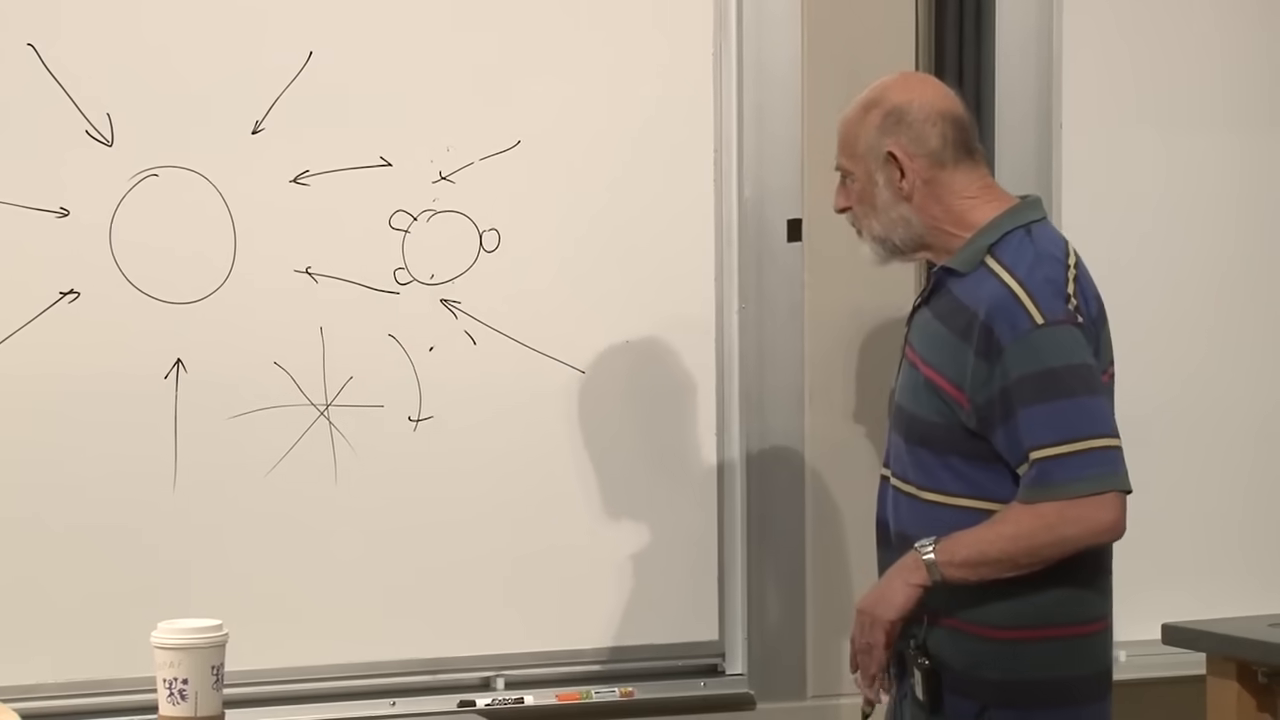
\includegraphics[width=\linewidth]{lecture_01_figure_09.png}
\caption{一个延展的自由下落物体同时表现出的径向拉伸和横向挤压。}
\par\smallskip
\textit{讲座时间点：00:47:55。}
\end{figure}

\begin{classroomqa}
\audiencequestion{潮汐力是否意味着等效原理失效？}
\lecturerresponse{它们决定了等效原理必须被表述得多么谨慎。在一个小到引力场在其范围内变化可忽略的系统中，可以通过自由下落参考系以相关精度消除引力。在更大系统中残余的变化就是潮汐场。\lecturetimestamp{00:48:08}}
\end{classroomqa}

\section{从闵可夫斯基几何到局部度规}

现在我们暂时离开引力稍作休息。闵可夫斯基早已教导我们，时空具有不变的局部几何。在一维空间中，取\(c=1\)，
\begin{equation}
 d\tau^2=dt^2-dx^2.
\label{eq:minkowski-proper-time}
\end{equation}
也可以改为定义\(ds^2=dx^2-dt^2=-d\tau^2\)。这一差别是号差约定，而不是物理上的差别。

\begin{classroomqa}
\audiencequestion{如果不把光速设为1，它应当出现在哪里？}
\lecturerresponse{如果\(t\)以时间单位测量，而\(x\)以长度单位测量，一种方便的形式是
\(d\tau^2=dt^2-dx^2/c^2\)。等价地，乘以\(c^2\)并使用
\(c^2d\tau^2=c^2dt^2-dx^2\)。选择\(ct\)或\(x/c\)作为坐标即可吸收该换算因子。\lecturetimestamp{00:51:02}}
\end{classroomqa}

\begin{figure}[H]
\centering
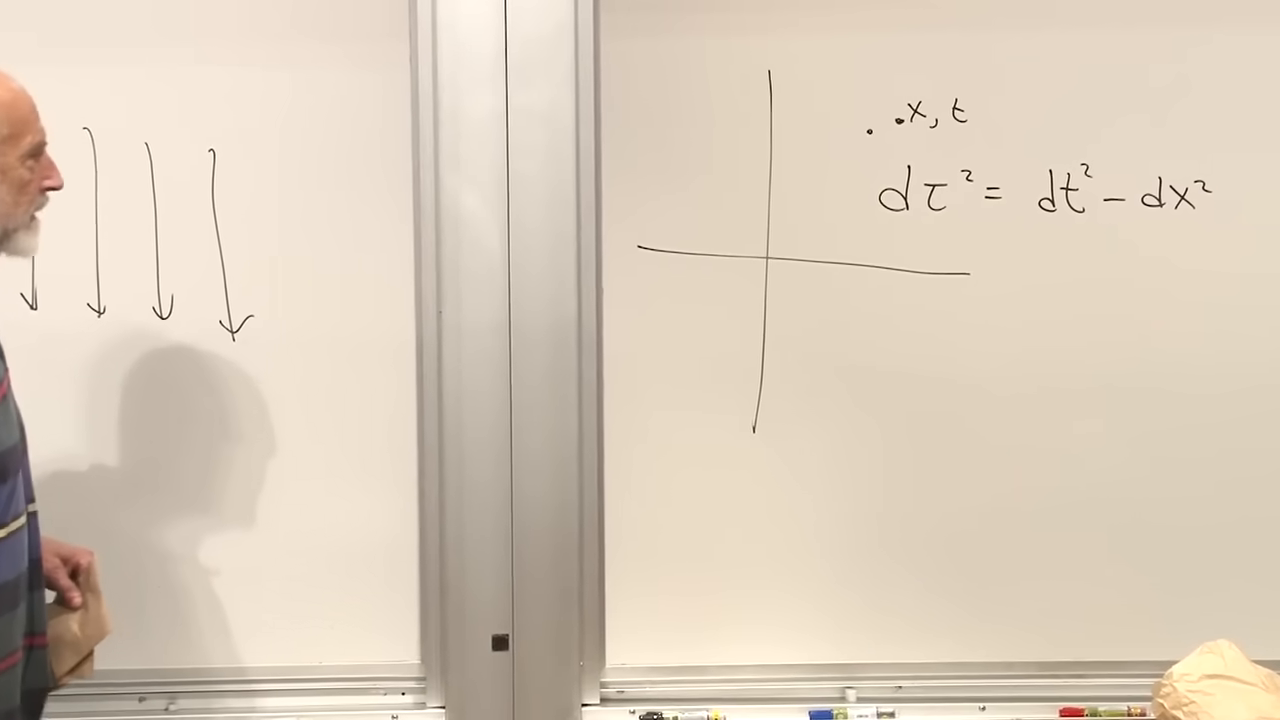
\includegraphics[width=\linewidth]{lecture_01_figure_10.png}
\caption{提供从狭义相对论到广义相对论之几何桥梁的固有时间隔。}
\par\smallskip
\textit{讲座时间点：00:51:10。}
\end{figure}

爱因斯坦认识到，判断一个引力场是否可被消除的问题，类似于高斯对曲面、黎曼对任意维数所研究的问题：给定一个局部距离定律，如何判断该几何是否真正弯曲？

在欧几里得笛卡儿坐标中，毕达哥拉斯给出
\begin{equation}
 ds^2=(dx^1)^2+(dx^2)^2+\cdots
     =\delta_{mn}\,dx^m dx^n.
\label{eq:euclidean-line-element}
\end{equation}
指标范围就是空间的维数。记号中没有任何东西会随坐标数是二、三还是二十六而改变。

\begin{figure}[H]
\centering
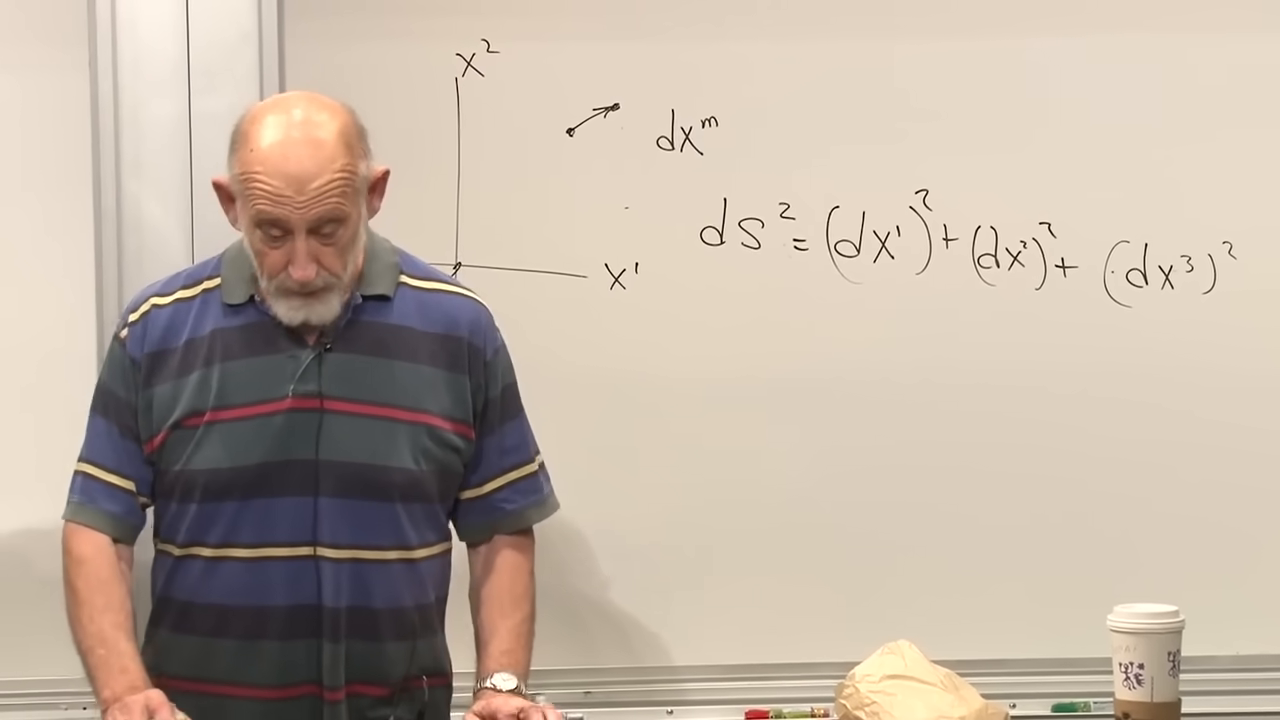
\includegraphics[width=\linewidth]{lecture_01_figure_11.png}
\caption{欧几里得线元作为坐标增量平方之和。}
\par\smallskip
\textit{讲座时间点：00:55:00。}
\end{figure}

在任意曲面上放置任意坐标\(x^m\)。相邻点之间的距离是二次型
\begin{equation}
 ds^2=g_{mn}(x)\,dx^m dx^n.
\label{eq:general-line-element}
\end{equation}
函数\(g_{mn}(x)\)是度规张量的分量。同一公式也适用于用曲线坐标描述的平坦曲面；度规分量不是常数本身并不能证明存在内禀曲率。

\begin{figure}[H]
\centering
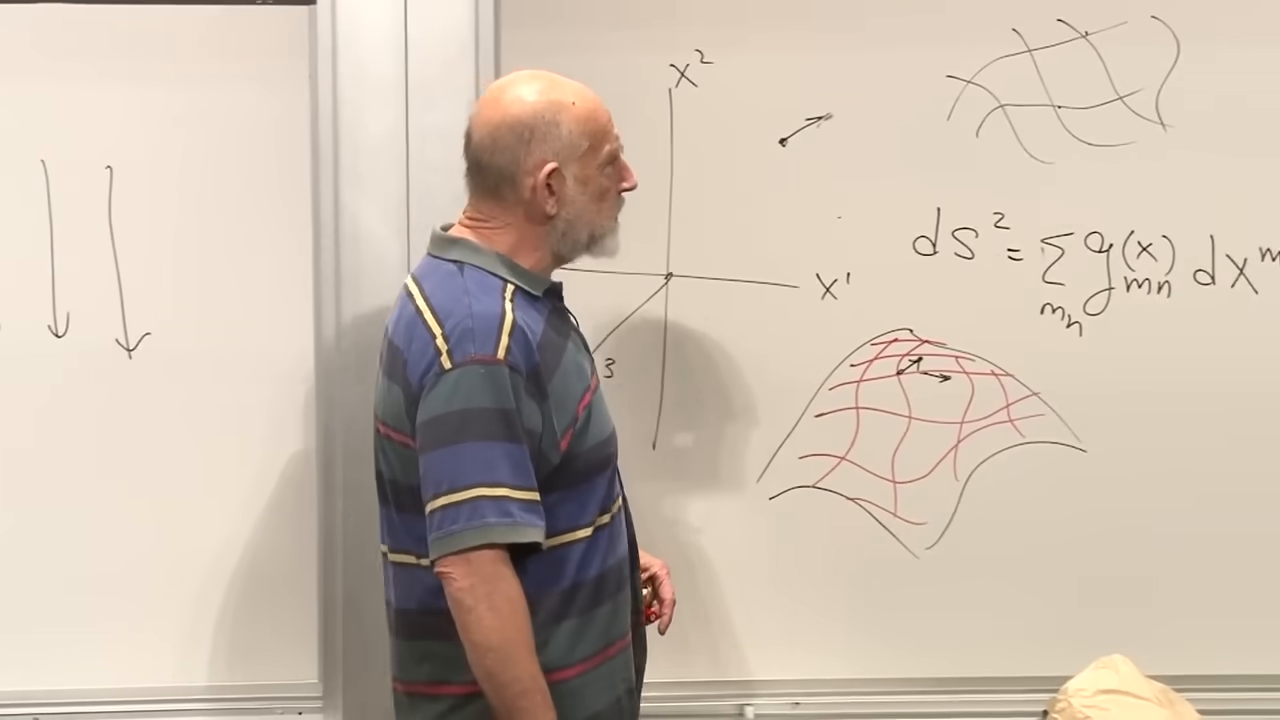
\includegraphics[width=\linewidth]{lecture_01_figure_12.png}
\caption{一般度规二次型与弯曲坐标网格并列。}
\par\smallskip
\textit{讲座时间点：00:58:20。}
\end{figure}

对于半径为\(R\)的球面，当\(\theta\)从极点量起时，
\begin{equation}
 ds^2=R^2\left(d\theta^2+\sin^2\theta\,d\phi^2\right).
\label{eq:sphere-polar}
\end{equation}
相同的经度增量在赤道附近覆盖很大的距离，而在极点附近覆盖很小的距离；这种位置依赖性正是该系数所记录的内容。

\begin{classroomqa}
\audiencequestion{通常的纬度是从赤道量起的，那么系数是否应当是余弦而不是正弦？}
\lecturerresponse{是的。如果\(\lambda\)表示从赤道量起的纬度，那么
\(ds^2=R^2(d\lambda^2+\cos^2\lambda\,d\phi^2)\)。
方程\eqref{eq:sphere-polar}使用的是从北极量起的极角
\(\theta=\pi/2-\lambda\)。
\lecturetimestamp{01:01:03}}
\end{classroomqa}

\begin{figure}[H]
\centering
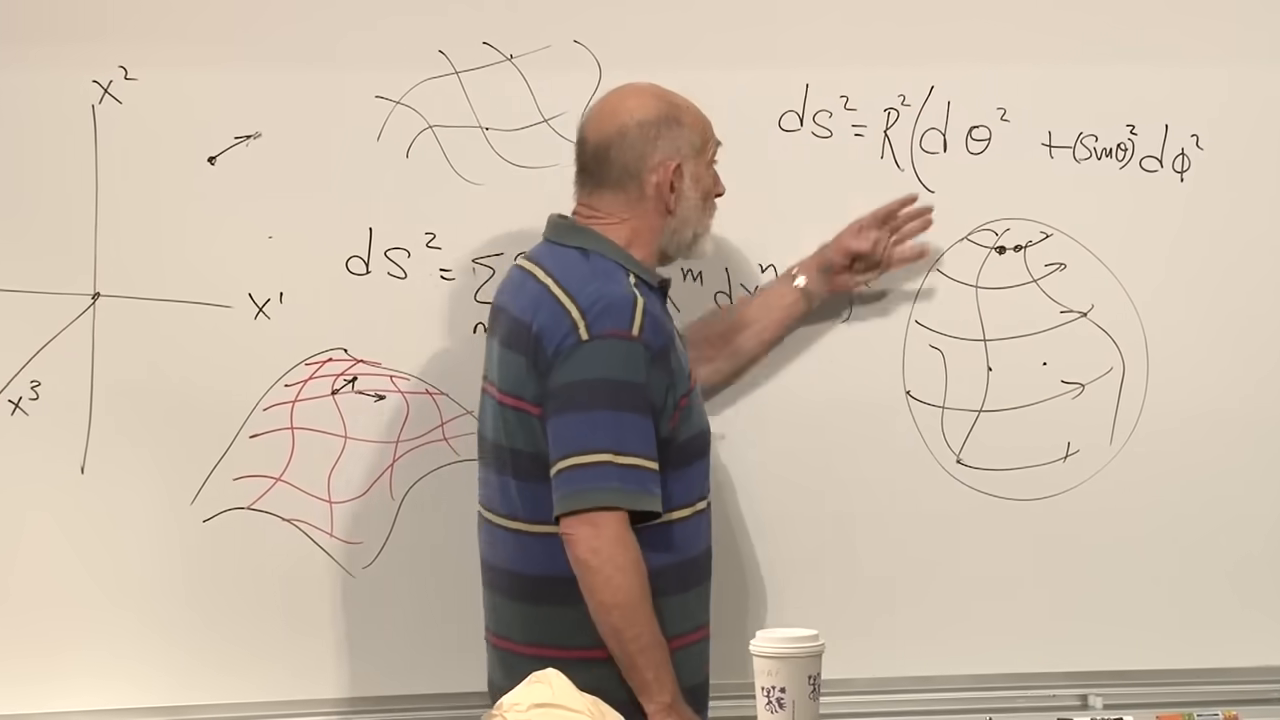
\includegraphics[width=\linewidth]{lecture_01_figure_13.png}
\caption{球面度规以及纬度--经度几何，后者确定了其依赖于位置的系数。}
\par\smallskip
\textit{讲义帧：01:00:30。}
\end{figure}

更一般的坐标可以引入\(d\theta\,d\phi\)交叉项，但局域距离在微分上仍是二次的。三次项或线性项不属于黎曼线元。

\section{局域距离与内禀曲率}

\begin{classroomqa}
\audiencequestion{度规公式是否也给出两个相距很远的点之间的距离？}
\lecturerresponse{不能通过直接代入得到。它给出的是相邻点之间的距离。宏观距离需要一条路径以及\(ds\)的积分；如果距离指的是最短路径，那么这条路径本身必须由几何求出。甚至可能有多条局部最短路径连接同一对端点。\lecturetimestamp{01:02:30}}
\end{classroomqa}

在凹凸不平的曲面上，想象在两个相距很远的点处钉上钉子，并在它们之间拉紧一根弦。这根弦可能绕过山丘的这一侧或另一侧，而移动山丘会改变最小化路径。全局距离取决于其间的几何。局域距离则更简单：度规在每一点提供一根小尺，几何由这些无穷小尺组装而成。

\begin{figure}[H]
\centering
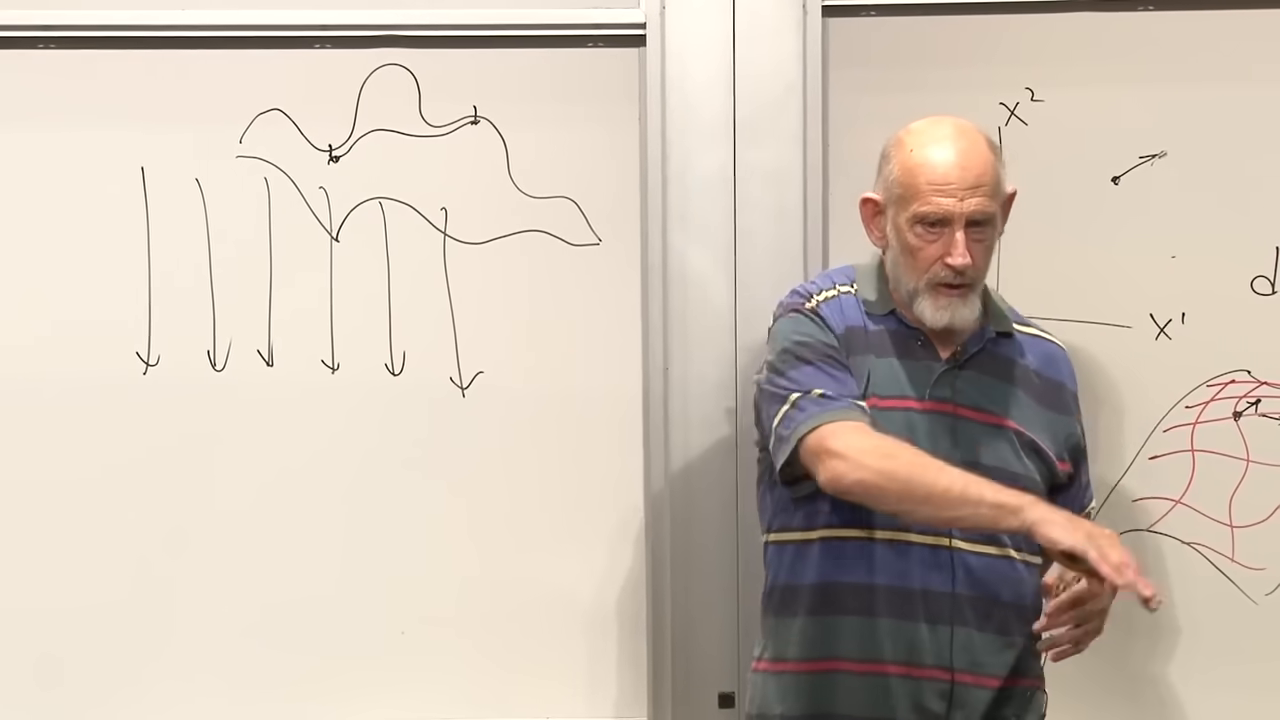
\includegraphics[width=\linewidth]{lecture_01_figure_14.png}
\caption{全局距离问题：一条拉紧的路径必须在其端点之间的曲面上穿行。}
\par\smallskip
\textit{讲义帧：01:04:00。}
\end{figure}

如果局域小块能够不拉伸、不撕裂地铺到平面上，那么内禀几何就是平坦的。具有三角化球面长度的小块无法在保持其边长的同时全部铺平。因此度规提出了一个精确的问题：给定\(g_{mn}(x)\)，能否判定它的无穷小小块能否像平坦空间那样拼合在一起？

\begin{figure}[H]
\centering
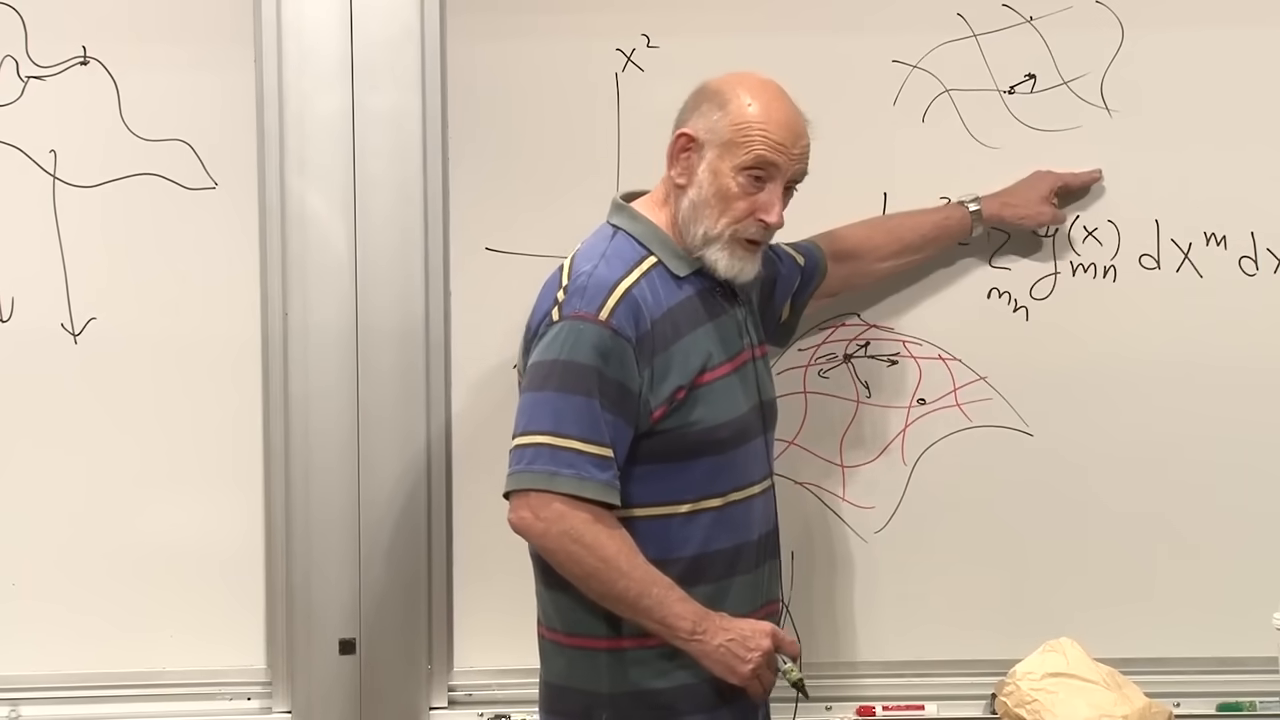
\includegraphics[width=\linewidth]{lecture_01_figure_15.png}
\caption{度规与局域坐标片被解释为组装几何所用的无穷小小块。}
\par\smallskip
\textit{讲义帧：01:05:20。}
\end{figure}

\begin{classroomqa}
\audiencequestion{能否通过测量周长与直径之比来诊断曲率？}
\lecturerresponse{可以，这是一个有用的二维检验。在弯曲曲面上，该比值可以不同于\(\pi\)。然而，对于无穷小圆，偏差以更高阶出现，而且该方法不像曲率张量那样能干净地推广。
\lecturetimestamp{01:07:26}}
\end{classroomqa}

如果存在一个坐标系使得在该区域内处处有
\begin{equation}
 g_{mn}=\delta_{mn},
\qquad
 ds^2=\delta_{mn}\,dx^m dx^n
\label{eq:flat-metric}
\end{equation}
，那么该区域就是平坦的。因此，一个复杂的\(g_{mn}(x)\)既可以描述弯曲空间，也可以仅仅描述平坦空间上的弯曲坐标。问题在于，坐标变换能否消除所有这些复杂性。

\begin{figure}[H]
\centering
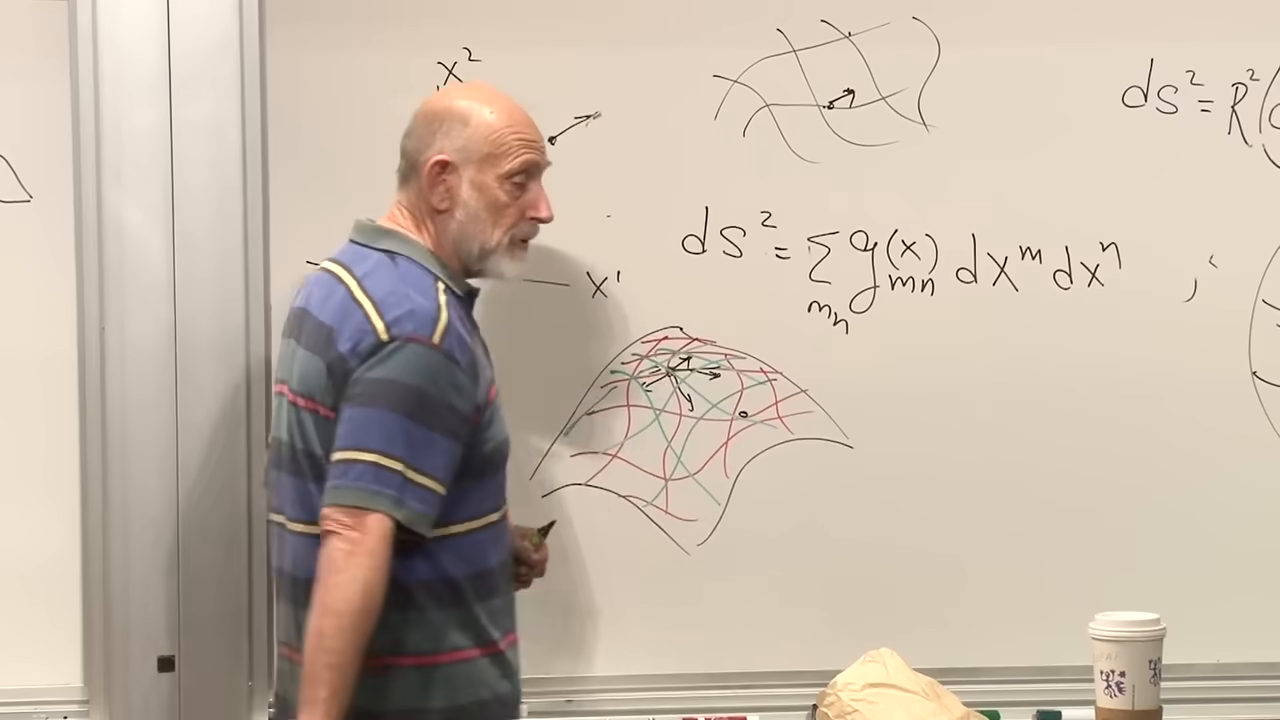
\includegraphics[width=\linewidth]{lecture_01_figure_16.png}
\caption{在局域坐标片上陈述的度规问题：它的曲线坐标形式能否变换为平坦形式？}
\par\smallskip
\textit{讲义帧：01:07:15。}
\end{figure}

\begin{classroomqa}
\audiencequestion{球面线元是否假设每个小间隔都是平坦的，尽管球面并非如此？}
\lecturerresponse{在最低阶，每个光滑曲面在一点处都由其切平面近似。曲率体现在相邻切平面近似如何无法拼合在一起，或者体现在跨越有限区域的高阶变化中。因此，局域欧几里得行为与全局曲率是相容的。\lecturetimestamp{01:10:01}}
\end{classroomqa}

\begin{classroomqa}
\audiencequestion{度规必须是连续的吗？在折痕或裂隙处会发生什么？}
\lecturerresponse{讨论假设坐标映射和度规足够光滑，以支持所需的导数。一张不拉伸而折叠的纸在折痕两侧具有相同的内禀距离；其引人注目的外观是外禀的。真正奇异或不光滑的几何需要单独处理，超出了这里使用的光滑框架。\lecturetimestamp{01:11:25}}
\end{classroomqa}

这一区分就是内禀几何。在三维空间中弯曲一页纸会改变其嵌入，但不会改变在纸面内测得的距离。一个被限制在纸面上、无法看到嵌入空间的生物，仍然可以测量其内禀几何。

\begin{figure}[H]
\centering
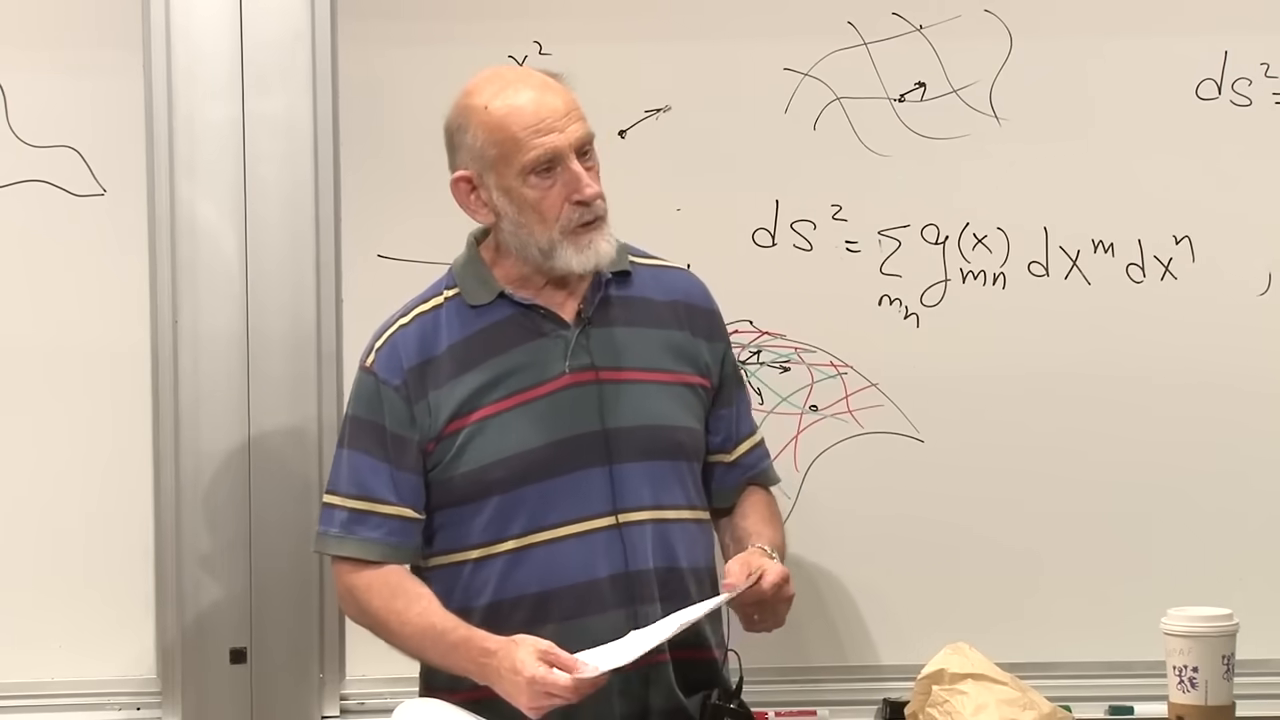
\includegraphics[width=\linewidth]{lecture_01_figure_17.png}
\caption{一张折叠的纸，用来把内禀距离与外显表象分离开来。}
\par\smallskip
\textit{讲义帧：01:13:00。}
\end{figure}

\begin{classroomqa}
\audiencequestion{为什么不干脆把度规对角化？}
\lecturerresponse{在任意一个点上，选取适当的坐标就能把度规对角化，并把它归一化为局部平坦形式。障碍在于要用同一个坐标系在整个区域内都做到这一点。仅靠考察单独一个点，是无法探测到曲率的。
\lecturetimestamp{01:13:48}}
\end{classroomqa}

\begin{figure}[H]
\centering
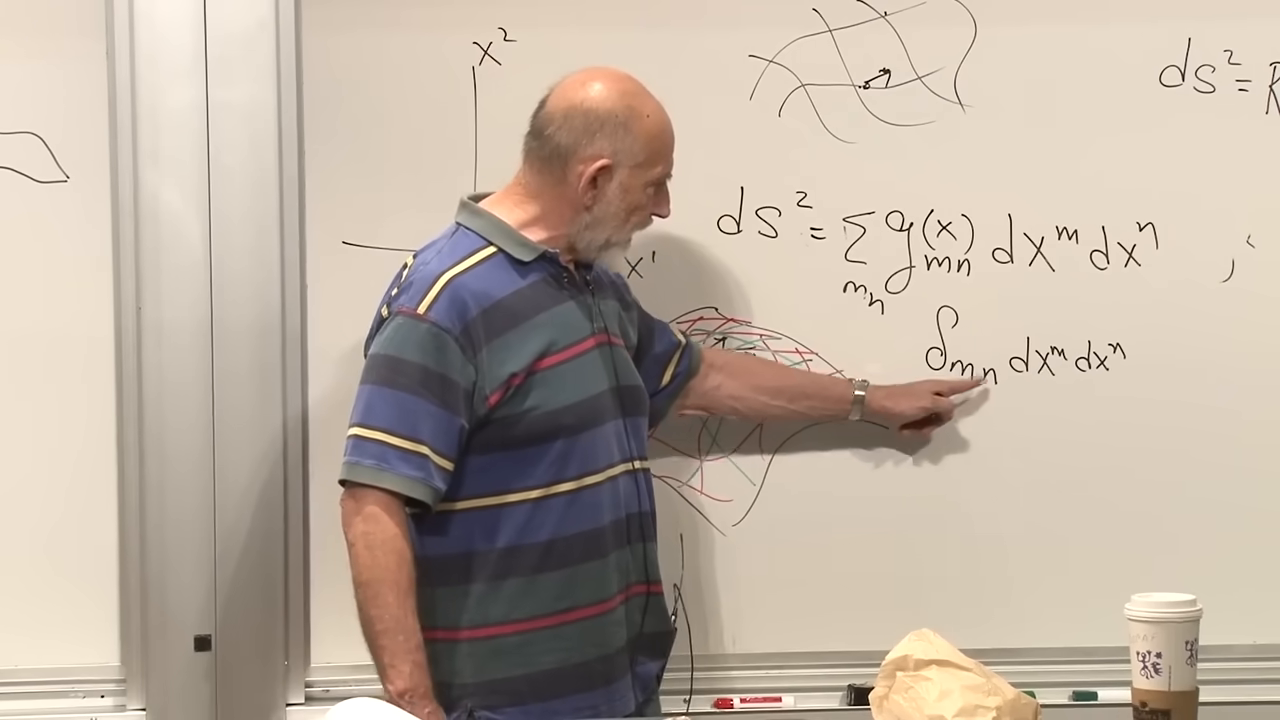
\includegraphics[width=\linewidth]{lecture_01_figure_18.png}
\caption{平坦的笛卡儿度规\(\delta_{mn}\)写在一般的局部二次型之下。}
\par\smallskip
\textit{讲义帧：01:16:00。}
\end{figure}

与引力的类比现在已是精确的，而不再只是提示性的。坐标力可以被消除，正如平坦空间的曲线坐标描述可以被消除一样。在广义相对论中，潮汐加速度由曲率来度量。用后来的记号来说，相邻的自由下落世界线满足测地偏离方程
\begin{equation}
 \frac{D^2\xi^\mu}{D\tau^2}
 =-R^\mu{}_{\nu\rho\sigma}
   u^\nu\xi^\rho u^\sigma.
\label{eq:geodesic-deviation-preview}
\end{equation}
曲率为零意味着不存在不变的潮汐场；曲率非零则意味着，无论怎样选取坐标，都无法在整个区域内消除引力。

\section{两个坐标系与一个矢量}

要判断一个度规能否变换为\(\delta_{mn}\)，我们必须首先知道几何对象如何变换。设\(x^m\)与\(y^m\)是同一区域上的两个光滑坐标系：
\begin{equation}
 x^m=x^m(y),\qquad y^m=y^m(x).
\label{eq:mutual-coordinate-maps}
\end{equation}
符号\(x\)与\(y\)标记的是完整的坐标系，而不是两个特定的空间方向。

\begin{figure}[H]
\centering
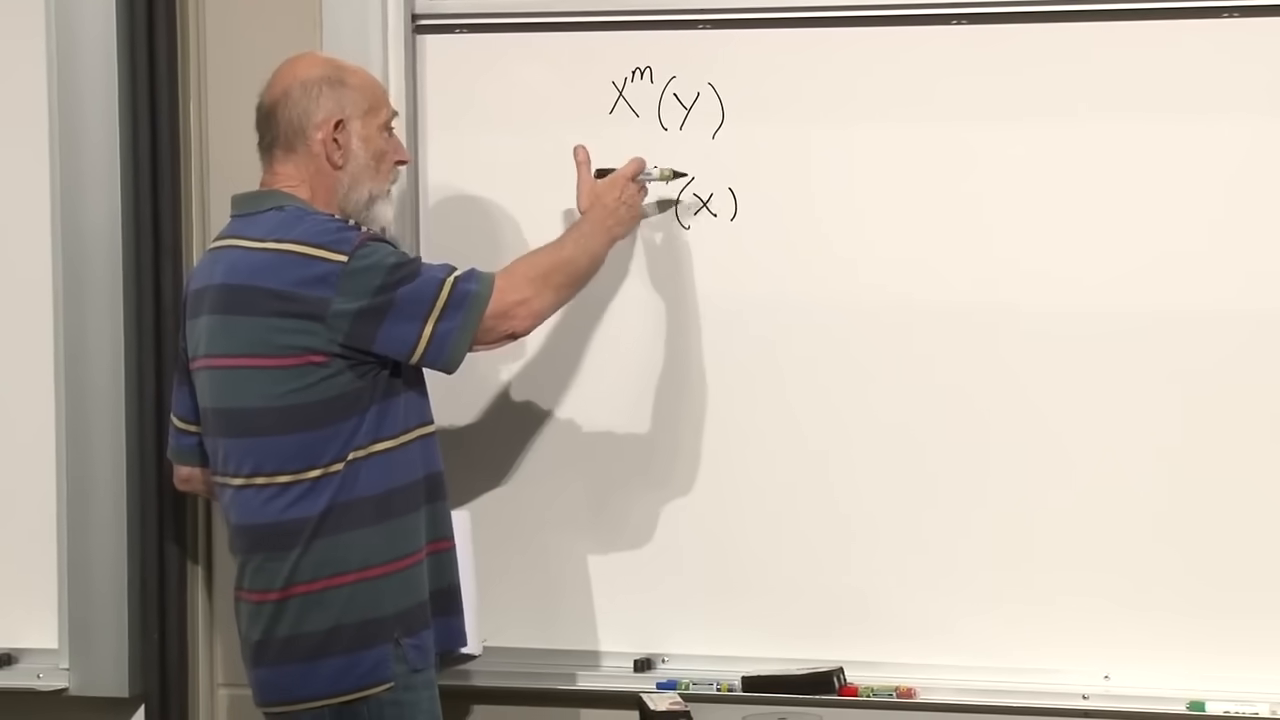
\includegraphics[width=\linewidth]{lecture_01_figure_19.png}
\caption{相互关联的坐标映射\(x^m(y)\)与\(y^m(x)\)。}
\par\smallskip
\textit{讲义帧：01:20:35。}
\end{figure}

对于相邻的点，链式法则给出
\begin{equation}
 dy^m=\frac{\partial y^m}{\partial x^p}\,dx^p.
\label{eq:differential-transform}
\end{equation}
重复指标\(p\)被求和。位移本身是一个几何矢量；\(dx^p\)与\(dy^m\)是它在两个坐标系中的分量。

\begin{figure}[H]
\centering
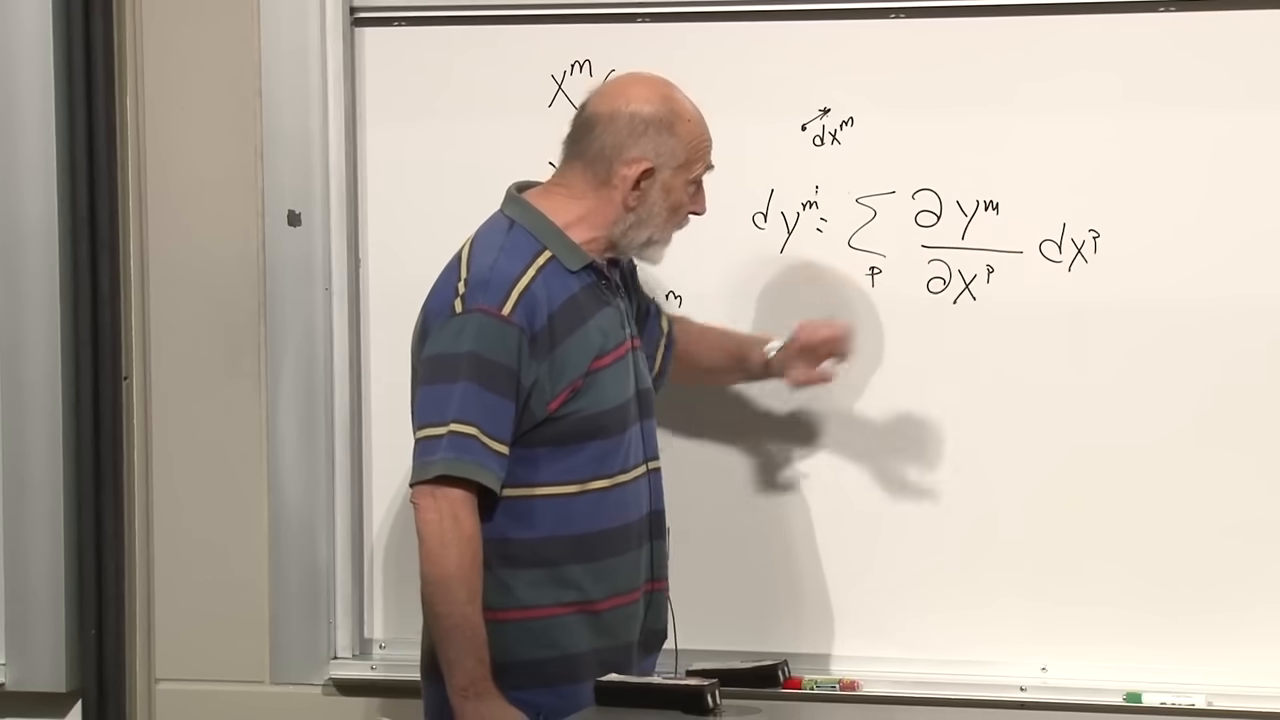
\includegraphics[width=\linewidth]{lecture_01_figure_20.png}
\caption{由链式法则得到的微分坐标变换。}
\par\smallskip
\textit{讲义帧：01:22:30。}
\end{figure}

\begin{classroomqa}
\audiencequestion{在曲线网格上，坐标线代表什么？}
\lecturerresponse{在二维情形下，固定一个坐标而让另一个坐标变化，就得到一条线。在更高维情形下，相应的常坐标集合是超曲面。它们的局部交线定义了用来分解矢量分量的坐标方向。\lecturetimestamp{01:25:20}}
\end{classroomqa}

逆变矢量由与坐标位移相同的变换律来定义：
\begin{equation}
 (V')^m(y)
 =\frac{\partial y^m}{\partial x^p}\,V^p(x).
\label{eq:contravariant-vector}
\end{equation}
沿曲面的速度就是一个例子。坐标改变时，矢量本身不变；改变的是它的分量。

\begin{figure}[H]
\centering
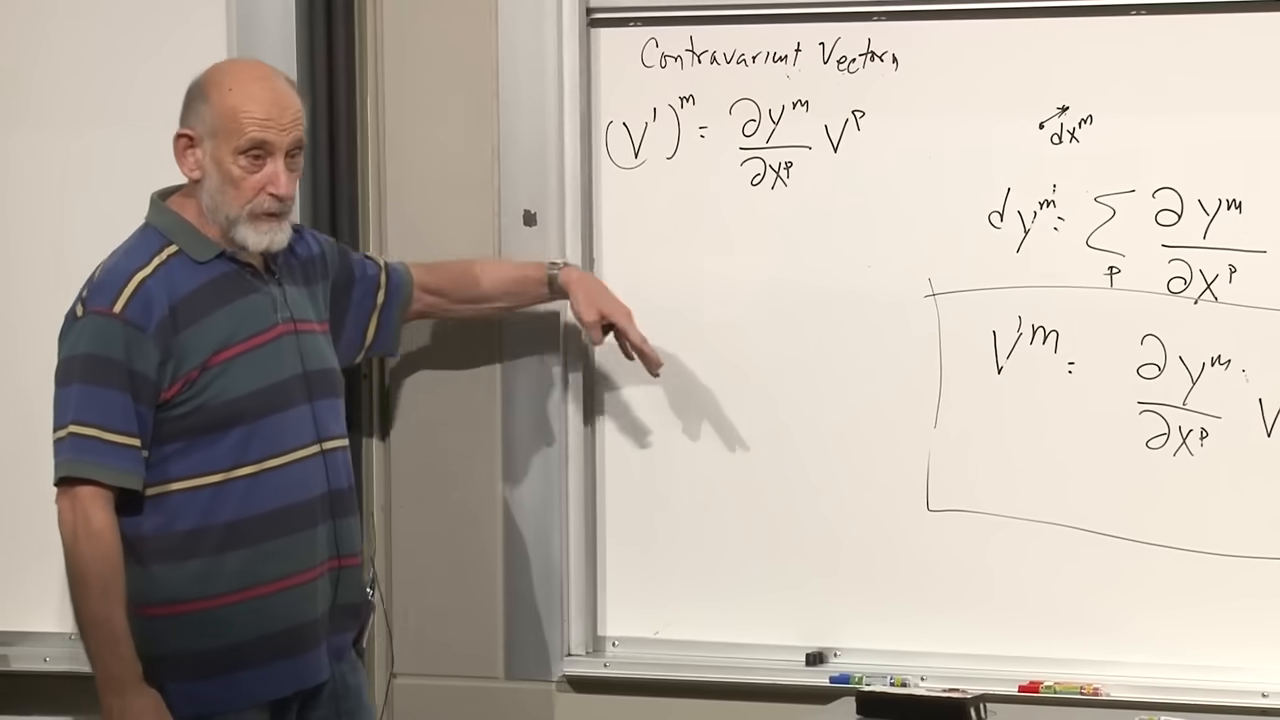
\includegraphics[width=\linewidth]{lecture_01_figure_21.png}
\caption{用方框标出的逆变矢量变换律。}
\par\smallskip
\textit{讲义帧：01:29:30。}
\end{figure}

爱因斯坦求和约定规定：只要一个指标在上方出现一次、在下方出现一次，就省略求和号。这一约定使公式更易于排印，但更重要的是，它让缩并的模式变得一目了然。

\begin{classroomqa}
\audiencequestion{关于允许使用哪些坐标系，是否作了什么特殊假设？}
\lecturerresponse{只假设这两个坐标系之间有函数关系，并且足够光滑，使得所写出的导数与逆映射在所讨论的区域内存在。并不假设线性性或正交性。\lecturetimestamp{01:28:12}}
\end{classroomqa}

\section{余矢量与链式法则}

设\(S(x)\)是一个标量：它在每一点都有一个确定的值，与坐标标记无关。温度和标量场就是例子。它的梯度具有分量
\begin{equation}
 W_p=\frac{\partial S}{\partial x^p}.
\label{eq:gradient-covector}
\end{equation}

\begin{figure}[H]
\centering
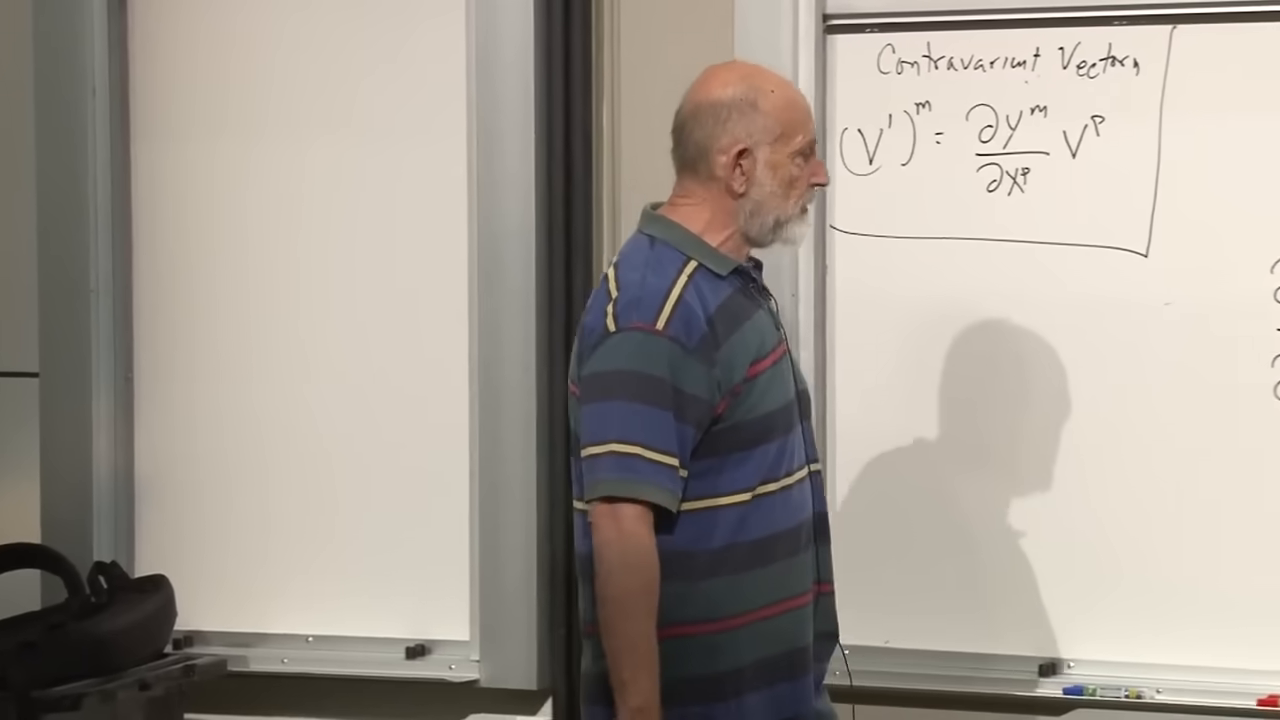
\includegraphics[width=\linewidth]{lecture_01_figure_22.png}
\caption{在逆变变换律旁边引入的标量梯度。}
\par\smallskip
\textit{讲义帧：01:31:40。}
\end{figure}

在\(y\)坐标中应用链式法则，
\begin{equation}
 W'_m
 =\frac{\partial S}{\partial y^m}
 =\frac{\partial x^p}{\partial y^m}
  \frac{\partial S}{\partial x^p}
 =\frac{\partial x^p}{\partial y^m}\,W_p.
\label{eq:covariant-vector}
\end{equation}
这就是协变矢量（即余矢量）的变换律。其雅可比矩阵是\eqref{eq:contravariant-vector}中那个雅可比矩阵的逆；因此，下指标与上指标编码了不同的变换行为。

\begin{figure}[H]
\centering
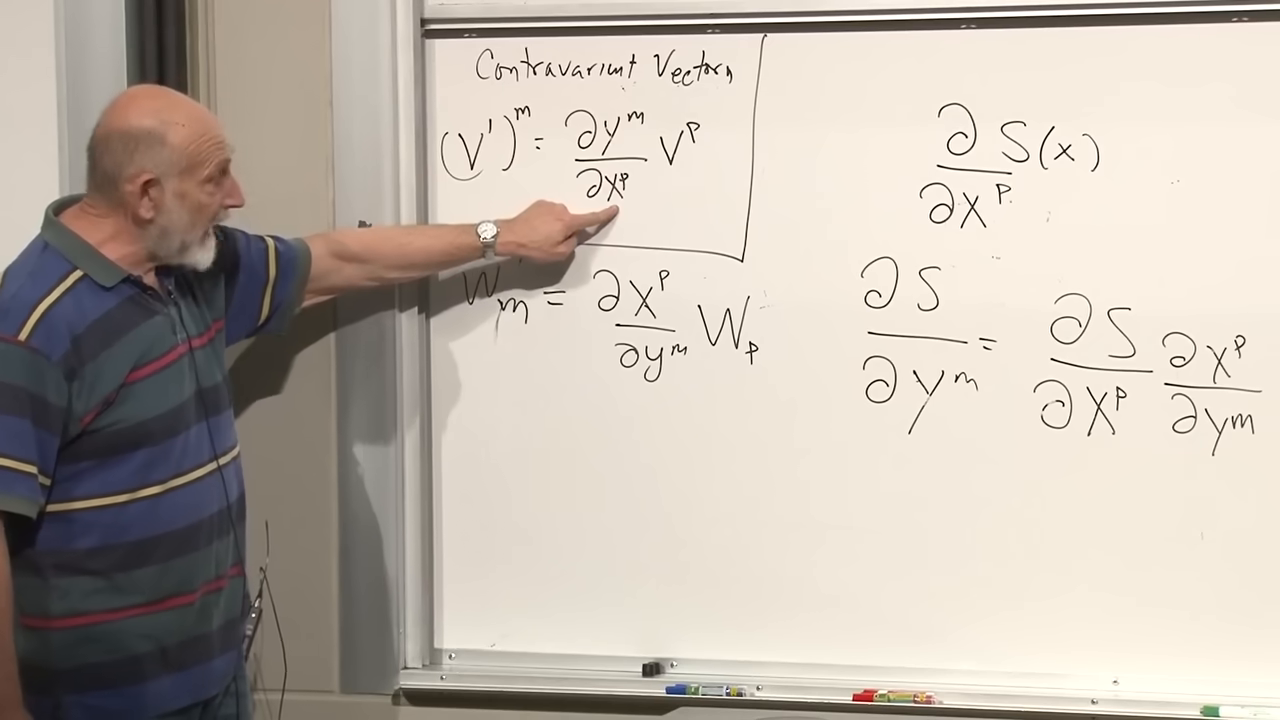
\includegraphics[width=\linewidth]{lecture_01_figure_23.png}
\caption{逆变与协变变换律并列展示。}
\par\smallskip
\textit{讲义帧：01:34:40。}
\end{figure}

\begin{classroomqa}
\audiencequestion{协变向量与逆变向量之间有什么联系？}
\lecturerresponse{在这个阶段，它们被定义为不同种类的对象：位移和速度以一种方式变换，梯度则以相反的方式变换。度规稍后将提供一种一一映射，用来降低或升高指标。在引入度规之前，不应假定这种关系。\lecturetimestamp{01:37:43}}
\end{classroomqa}

\begin{classroomqa}
\audiencequestion{此前降低指标是否改变了时间分量的符号？}
\lecturerresponse{那个符号来自洛伦兹度规。目前的推导首先是在普通欧几里得几何中进行的。升高或降低指标总是使用相应的度规；只有当该度规具有洛伦兹号差时，才会出现时间分量的符号。
\lecturetimestamp{01:38:29}}
\end{classroomqa}

\begin{classroomqa}
\audiencequestion{是否应当已经把这两条变换律视为同一个向量的两种分量描述？}
\lecturerresponse{还不能。一旦有了度规，逆变向量\(V^m\)就可以转换为余向量\(V_m=g_{mn}V^n\)。在建立该映射之前，上指标对象与下指标对象在逻辑上是不同的。\lecturetimestamp{01:39:00}}
\end{classroomqa}

这些公式与维数无关。指标范围会改变，但变换律不会。

\section{具有多于一个指标的张量}

取两个逆变向量\(V^m\)和\(U^n\)。它们的乘积
\begin{equation}
 T^{mn}=V^mU^n
\label{eq:rank-two-product}
\end{equation}
是一个二阶逆变张量。在三维中它有九个分量；在四维中它有十六个。除非另外给出对称性，否则指标的次序很重要：\(T^{mn}\)不必等于\(T^{nm}\)。

\begin{figure}[H]
\centering
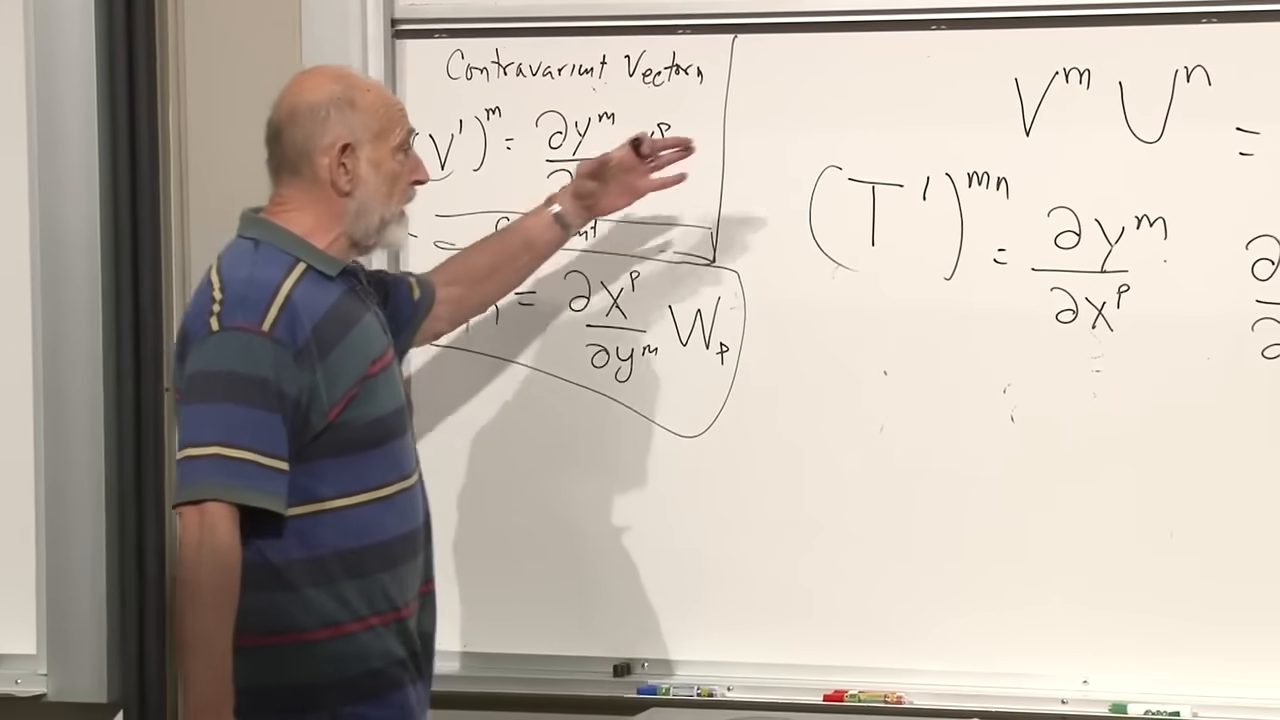
\includegraphics[width=\linewidth]{lecture_01_figure_24.png}
\caption{一个由两个逆变向量的乘积构成的二阶张量。}
\par\smallskip
\textit{讲义帧：01:43:40。}
\end{figure}

每个上指标贡献一个正向雅可比因子：
\begin{equation}
 (T')^{mn}
 =\frac{\partial y^m}{\partial x^p}
  \frac{\partial y^n}{\partial x^q}
  T^{pq}.
\label{eq:rank-two-contravariant}
\end{equation}
乘积构造给出了这条规则的动机，但变换律才是张量的定义。一个三阶逆变张量将获得三个这样的雅可比因子。

\begin{figure}[H]
\centering
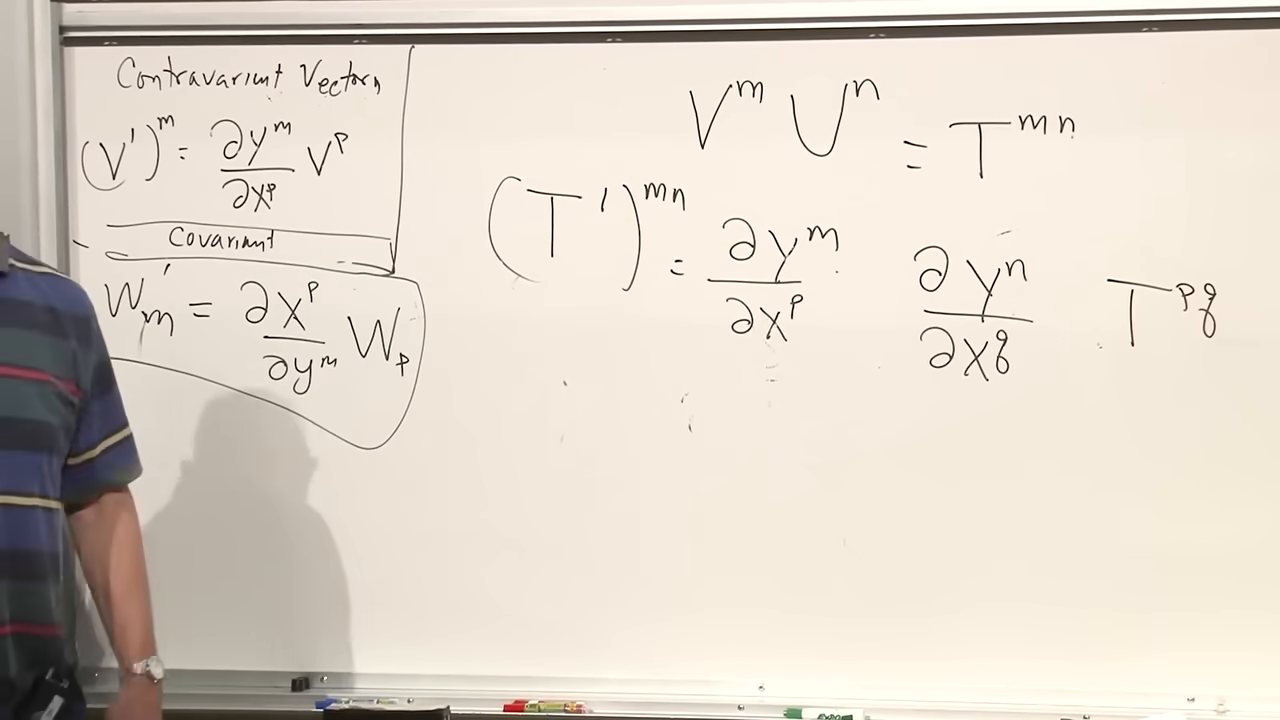
\includegraphics[width=\linewidth]{lecture_01_figure_25.png}
\caption{\(T^{mn}\)的变换中的两个雅可比因子。}
\par\smallskip
\textit{讲义帧：01:44:20。}
\end{figure}

同样，每个下指标贡献一个逆雅可比因子：
\begin{equation}
 T'_{mn}
 =\frac{\partial x^p}{\partial y^m}
  \frac{\partial x^q}{\partial y^n}
  T_{pq}.
\label{eq:rank-two-covariant}
\end{equation}
混合张量则各使用一个这样的因子。

\begin{figure}[H]
\centering
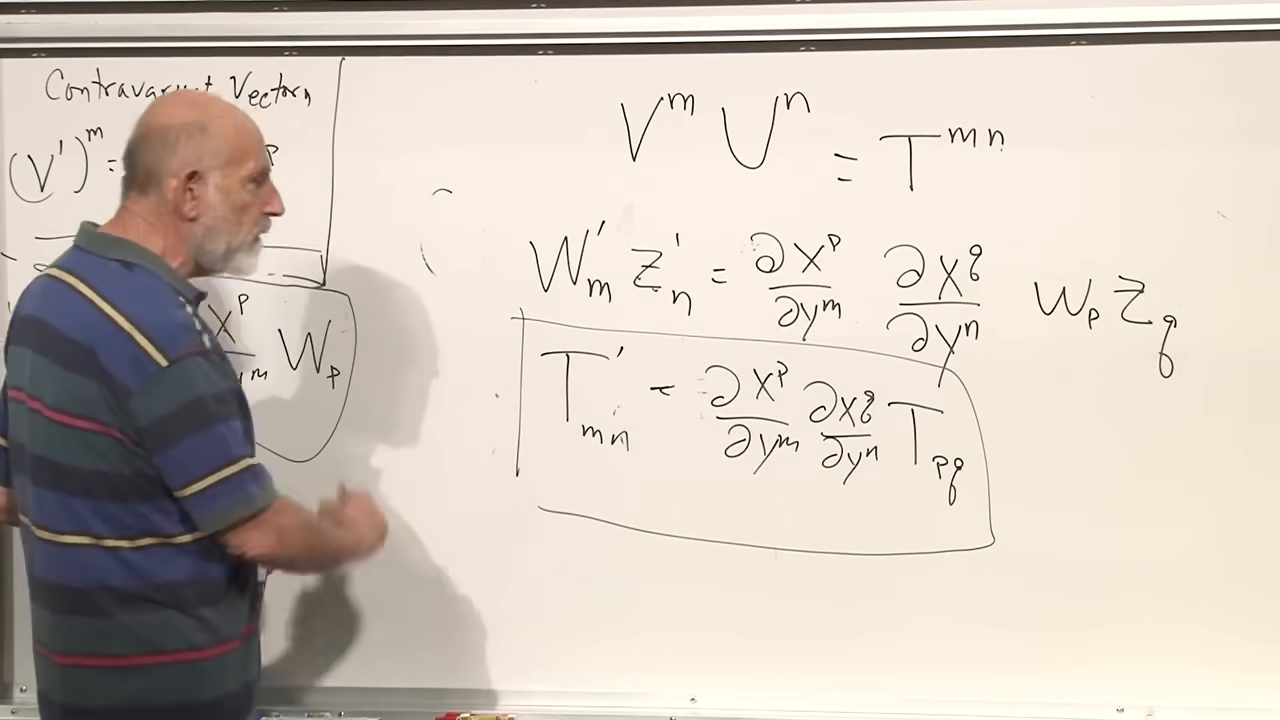
\includegraphics[width=\linewidth]{lecture_01_figure_26.png}
\caption{具有两个协变指标的张量的完整变换律。}
\par\smallskip
\textit{讲义帧：01:47:30。}
\end{figure}

同样的变换机制现在适用于度规。由于间隔是标量，它在任一坐标系中都必须具有相同的值：
\begin{align}
 ds^2
 &=g_{mn}(x)\,dx^m dx^n,\\
 dx^m
 &=\frac{\partial x^m}{\partial y^p}\,dy^p.
\end{align}
代入后补全了黑板上未写完的那一行：
\begin{equation}
 g'_{pq}(y)
 =\frac{\partial x^m}{\partial y^p}
  \frac{\partial x^n}{\partial y^q}
  g_{mn}(x(y)).
\label{eq:l1-metric-transformation}
\end{equation}
因此\(g_{mn}\)是一个二阶协变张量。

\begin{figure}[H]
\centering
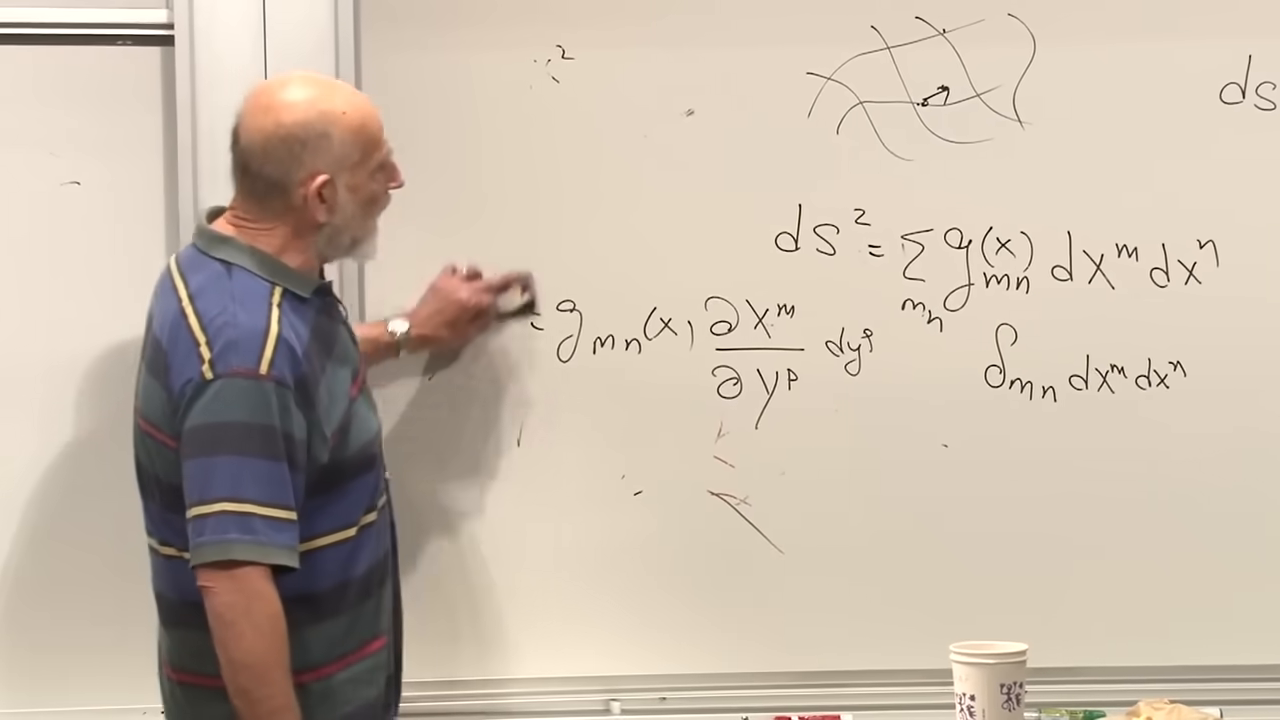
\includegraphics[width=\linewidth]{lecture_01_figure_27.png}
\caption{在讲座结束时从线元的不变性出发所开始的度规变换。}
\par\smallskip
\textit{讲义帧：01:48:40。}
\end{figure}

开头提出的物理问题现在变成了一个数学问题。给定\(g_{mn}(x)\)，是否存在一个坐标变换，使得在该区域内处处有\(g'_{mn}=\delta_{mn}\)？如果存在，那么表面的复杂性只是坐标的复杂性。如果不存在，那么障碍就是曲率，而在时空中，这个障碍就是引力的不变量内容。
